% DataAcquisitionSystem.tex
\section{Data Acquisition System}

% % for code listings
% \begin{lstlisting}[style=cstyle, caption=System Architecture Code Example, label=lst:SystemArchitecture8]
% # Your code here
% \end{lstlisting}

% % for figures
% \begin{figure}[htbp] %h-ere t-op b-ottom p-page (separate) -good to allow all htbp to give the compiler more options
%     \centering
%     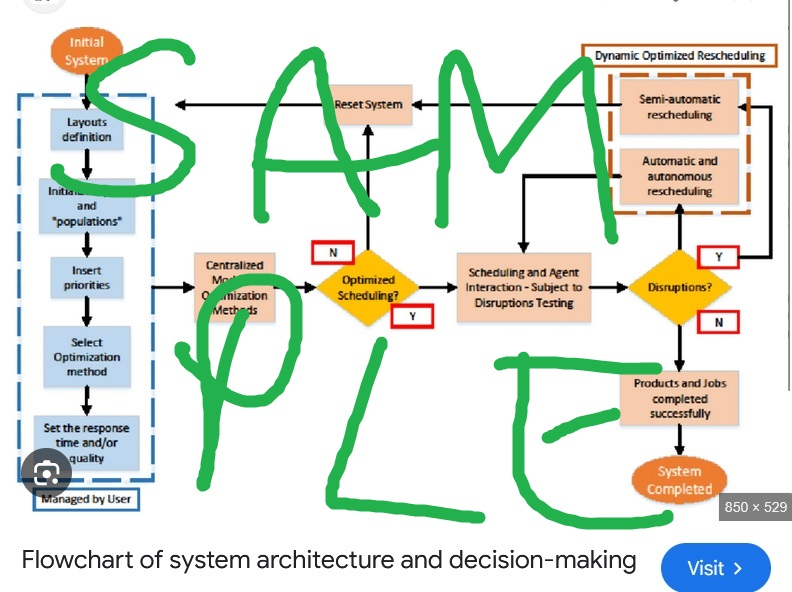
\includegraphics[width=0.6\textwidth]{figures/methodology/system_architecture.jpg}
%     \caption{System Architecture Diagram}
%     \label{fig:system-architecture3}
% \end{figure}

% % Include a flowchart in TEX mode
% \begin{figure}[H]
%     \centering
%     \scalebox{0.8}{ % Scale to 80% of original size
%         % try generating flowcharts as svg in Claude 
% and edit with inkscape instead of this.
% but claude did generate this one so might 
% be useful too but you can't easily make
% small repairs in inkscape


% CNN Transfer Learning Flowchart - Compact Multi-Column Layout
% \begin{figure}[htbp]

\centering
\resizebox{\textwidth}{!}{ % Scale to fit width while maintaining aspect ratio
\begin{tikzpicture}[node distance=0.8cm and 1.5cm, auto]
    % Define a smaller block style
    \tikzset{
      block/.style = {rectangle, draw, fill=blue!20, 
                      text width=7em, text centered, rounded corners, minimum height=1.8em, font=\small},
    }
    
    % Brazilian model training - Column 1
    \node [block] (brazildata) {Download Brazilian coins dataset};
    \node [block, below=of brazildata] (extract) {Extract dataset};
    \node [block, below=of extract] (setup) {Setup directories};
    \node [block, below=of setup] (define) {Define train/val dirs};
    \node [block, below=of define] (create) {Create CNN architecture};
    \node [block, below=of create] (compile) {Compile the CNN};
    \node [block, below=of compile] (train) {Train model};
    \node [block, below=of train] (trained) {Model trained (5 classes)};
    
    % Transfer learning - Column 2 (Middle)
    \node [block, right=2.5cm of brazildata] (freeze) {Freeze all layers};
    \node [block, below=of freeze] (replace) {Replace final layers};
    \node [block, below=of replace] (add) {Add regularization and dropout};
    \node [block, below=of add] (output) {New output layer (8 classes)};
    \node [block, below=of output] (finaltrain) {Train and fine-tune};
    \node [block, below=of finaltrain] (inference) {Perform inference on new coins};
    
    % UK data preparation - Column 3 (Right)
    \node [block, right=2.5cm of freeze] (ukdata) {Download UK coins dataset};
    \node [block, below=of ukdata] (ukextract) {Extract UK dataset};
    \node [block, below=of ukextract] (uksetup) {Setup UK directories};
    \node [block, below=of uksetup] (ukgen) {Create data generators (80/20 split)};
    
    % Connect all nodes with arrows
    \path [line] (brazildata) -- (extract);
    \path [line] (extract) -- (setup);
    \path [line] (setup) -- (define);
    \path [line] (define) -- (create);
    \path [line] (create) -- (compile);
    \path [line] (compile) -- (train);
    \path [line] (train) -- (trained);
    
    \path [line] (ukdata) -- (ukextract);
    \path [line] (ukextract) -- (uksetup);
    \path [line] (uksetup) -- (ukgen);
    
    % Connect the columns
    \path [line] (trained) -- node[midway, above] {Transfer} (freeze);
    \path [line] (ukgen) |- (finaltrain);
    
    % Connect middle column
    \path [line] (freeze) -- (replace);
    \path [line] (replace) -- (add);
    \path [line] (add) -- (output);
    \path [line] (output) -- (finaltrain);
    \path [line] (finaltrain) -- (inference);
    
    % Group boxes to show different stages with smaller padding
    \begin{pgfonlayer}{background}
        \node[group={[yshift=0.3cm]above:Brazilian Model Training}, fit={(brazildata) (extract) (setup) (define) (create) (compile) (train) (trained)}, inner sep=0.2cm] {};
        \node[group={[yshift=0.3cm]above:UK Data Preparation}, fit={(ukdata) (ukextract) (uksetup) (ukgen)}, inner sep=0.2cm] {};
        \node[group={[yshift=0.3cm]above:Transfer Learning}, fit={(freeze) (replace) (add) (output) (finaltrain) (inference)}, inner sep=0.2cm] {};
    \end{pgfonlayer}
\end{tikzpicture}
}
% \caption{CNN Transfer Learning Flowchart: Brazilian to UK Coins}
% \label{fig:cnn-flowchart}
% \end{figure} % \input is for tex files \includegraphics is for images
%     }
%     \caption{System Design Overview Flowchart}
%     \label{fig:decriptiveLabel22} % descriptive to call in text with \ref{fig:decriptiveLabel22}
% \end{figure}


% other subsections
\subsection{Functional Requirements}
% Your content here
The output signal from the photodiode array amplifier is required to be converted to digital form for post-processing. This requirement is filled by designing a Digital Acquisition System (DAQ) capable of recording the signal from the four photodiode circuits simultaneously.
The choice of design was conceived by analysing the analog signal and determining some basic requirements of the Analog to Digital Converter (ADC) the DAQ must possess. 
%
% ANALOG SIGNAL CHARACTERISTICS
%
\paragraph{Analog Signal Characteristics}
\begin{itemize}
    \item The signal is four channel, one per photodiode, and between 0 and 5 Volts, as the TIA and post amplification was designed specifically for this output.
    \item Close to DC frequency, i.e., static in nature, due to light intensity remaining static under most tests. One test is performed at 0.2Hz, which is still still very low frequency, with the light completing a semicircular arc once in 130 seconds (26 positions of 5 seconds each). 
    \item Later in testing it was found that the signal is impacted by interference of 400mVpp at a frequency fluctuating from 160kHz to 180kHz from the RED testbench power supply, as pictured in Figure~\ref{fig:sigNoise}.
\end{itemize}
% Noise figure
\begin{figure}[htbp] 
    \centering
    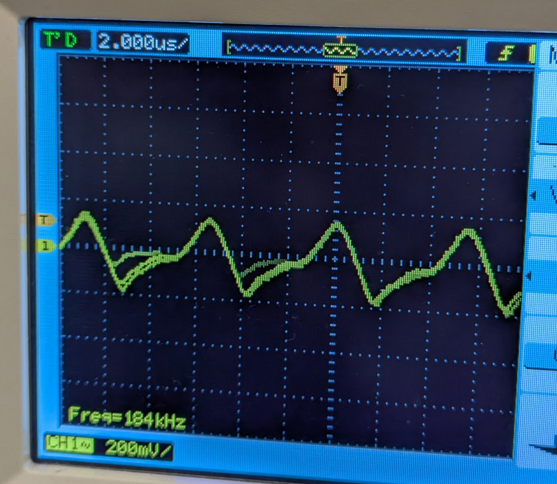
\includegraphics[width=0.4\textwidth]{chapters/methodology/ArduinoDAQ/signal_noise.png}
    \caption{Signal Noise Analysis, oscilloscope AC coupled}
    \label{fig:sigNoise}
\end{figure}
%
%     CSV DATA STRUCTURE
%
\paragraph{CSV Data Structure and Format Specification}is as follows:

The output of the DAQ is to be saved in Comma Separated Values (CSV) file format, with columns as follows: Sample(nr.), Time(ms), A0(V), A1(V), A2(V), A3(V). This allows for easy post-processing and plotting.
\subsection{Design Approach}
The characteristics of the signal being low frequency, combined with the requirement to read all four signals simultaneously and in sync, meant two things: the Sampling Rate could be quite low due to Nyquist theorem telling us that the sampling rate must be at least twice the frequency of the signal being sampled, in order to maintain the original signal without aliasing~\cite[p. 146]{RefWorks:oppenheim2013discrete-time}. Therefore a low performing ADC is acceptable for a signal changing at under 1Hz. And secondly, the DAQ must support sampling from at least four analog inputs. These requirements meant that a cheap Arduino based DAQ could fit perfectly the needs of the project: it is powered by the Atmega328P which has an included ADC of 15 ksps~\cite[p.205]{RefWorks:atmel2015atmega328p}. And the Arduino Nano has four analog inputs. 
\subsubsection{Arduino Programming}
The Arduino-based DAQ will require both a C++ program written for the Arduino itself, as well as a program or script on the PC receiving the digitized signal, this is because the Arduino lacks both the memory requirements and capability to store the recorded digitized signal to some internal memory.
\paragraph{The Arduino C++ Program} must be able to listen to commands from the user on the PC receiving, start a recording, and immediately transmit to the PC over serial communication. 

\subsection{Technical Specifications}


\subsubsection{Arduino Code}
The Arduino Code which uses the Arduino ADC is formed of the setup() function triggered once at the start/reset of the device and a standard continuous loop triggered after setup completes. Inside the loop, two if statements check for instructions from the PC script. The recording time limit is hardcoded as a global function. Figure~\ref{fig:arduinoPseudoCodeFlowchart} shows the algorithm as a Flowchart that checks for Serial data in, waits for a command to start recording, and if recording time has reached the preset limit, it stops recording, sends the last values to the Python script on the PC and a "recording\_stopped" command. A FSM diagram is also available in Figure~\ref{fig:arduinoFSM}. The pseudocode used while designing the Arduino side of the DAQ system, is available in Listing~\ref{lst:arduinoPseudoCode}. The final code is available in Appendix \ref{subsec:arduinoCppcode}.
\paragraph{The Atmega328P} does not have a separate ADC clock input, therefore the CPU clock is used by first dividing by a default rate of 128, this divider is changed to 16 by changing bits 2-0 to 100, as per~\cite[p.219]{RefWorks:atmel2015atmega328p}. This increases the clock speed available to the ADC for a higher sampling rate. This results in a 1MHz clock signal to the ADC (16MHz/16) which seemed needed when dealing with multiplexing four analog inputs to a single ADC. The process is as follows:


Original ADC Clock Speed (with default prescaler of 128):
\begin{equation} \label{origclk}
  \begin{split}
f_\text{ADC-default} = \frac{f_\text{CPU}}{Prescaler_\text{default}} = \frac{16 \text{ MHz}}{128} = 125 \text{ kHz}
  \end{split}
\end{equation}
\addequation{Default ADC Clock Frequency Calculation}

Optimized ADC Clock Speed (with modified prescaler of 16):
\begin{equation} \label{optimizedclk}
  \begin{split}
f_\text{ADC-optimized} = \frac{f_\text{CPU}}{Prescaler_\text{optimized}} = \frac{16 \text{ MHz}}{16} = 1 \text{ MHz}
\end{split}
\end{equation}
\addequation{Optimized ADC Clock Frequency Calculation}

Conversion Time Calculations:
ADC requires approximately 13 clock cycles for each conversion~\cite[p.208]{RefWorks:atmel2015atmega328p}
Optimized ADC Clock Speed (with modified prescaler of 16):
\begin{equation} \label{optimCLKspeed}
  \begin{split}
T_\text{conversion-default} = 13 \times \frac{1}{f_\text{ADC-default}} = 13 \times \frac{1}{125 \text{ kHz}} \approx 104 \text{ $\mu$s}
  \end{split}
\end{equation}
\addequation{Default ADC Conversion Time}

\begin{equation} \label{optimCLKspeed2}
  \begin{split}
T_\text{conversion-optimized} = 13 \times \frac{1}{f_\text{ADC-optimized}} = 13 \times \frac{1}{1 \text{ MHz}} \approx 13 \text{ $\mu$s}
  \end{split}
\end{equation}
\addequation{Optimized ADC Conversion Time}

Time required to sample all 4 analog inputs:
\begin{equation} \label{T4analogIn}
  \begin{split}
T_\text{4channels-default} = 4 \times T_\text{conversion-default} = 4 \times 104 \text{ $\mu$s} \approx 416 \text{ $\mu$s}
\end{split}
\end{equation}
\addequation{Total Sampling Time for 4 Channels (Default)}

\begin{equation} \label{T4analogIn2}
  \begin{split}
T_\text{4channels-optimized} = 4 \times T_\text{conversion-optimized} = 4 \times 13 \text{ $\mu$s} \approx 52 \text{ $\mu$s}
\end{split}
\end{equation}
\addequation{Total Sampling Time for 4 Channels (Optimized)}

Maximum theoretical sampling frequency for all 4 channels:
\begin{equation} \label{Tmax4ch}
  \begin{split}
f_\text{sampling-max-default} = \frac{1}{T_\text{4channels-default}} = \frac{1}{416 \text{ $\mu$s}} \approx 2.4 \text{ kHz}
\end{split}
\end{equation}
\addequation{Maximum Theoretical Sampling Frequency (Default)}

\begin{equation} \label{Tmax4ch2}
  \begin{split}
f_\text{sampling-max-optimized} = \frac{1}{T_\text{4channels-optimized}} = \frac{1}{52 \text{ $\mu$s}} \approx 19.2 \text{ kHz}
\end{split}
\end{equation}
\addequation{Maximum Theoretical Sampling Frequency (Optimized)}

Actual limited sampling frequency (based on minSampleInterval = 2ms):
\begin{equation} \label{Tlim2ms}
  \begin{split}
f_\text{sampling-actual} = \frac{1}{2 \text{ ms}} = 500 \text{ Hz} \text{ per channel}
\end{split}
\end{equation}
\addequation{Actual Limited Sampling Frequency}

Effective data rate across all channels:
\begin{equation} \label{EffectiveDATArate}
  \begin{split}
\text{Data Rate} = 4 \text{ channels} \times 500 \text{ Hz} = 2000 \text{ samples/second}
\end{split}
\end{equation}
\addequation{Total Effective Data Rate}
In real testing the actual sampling rate was closer to 330Hz for 5 second recordings or 100Hz for a 2 minute recording - after some investigation the only explanation was the relatively small size of the transmission buffer implemented by the Serial C++ library. The buffer is of only 64 bytes, and when it fills, the function Serial.write() (used by println() ) will block the write until there is space in the buffer[ref:arduino.cc/serial.write]. As our line of text is quite long "498,5000,0.059,0.054,0.073" for example has 26 characters (last line of a 5 second recording). For larger recording length, where the first and second column, Sample and Time, can get quite large, the sampling rate decreased considerably, but was kept constant (around 10ms for a 2 minute recording). Presumably due to optimization in the Arduino Serial Hardware/Software or compiler, it remains constant at 10ms. However this was not investigated further as for our near-DC signal, even 10ms was a fast enough sampling rate for our DC-like signal.


% Flowchart Arduino Code
\begin{figure}[p] %h-ere t-op b-ottom p-page (separate) -good to allow all htbp to give the compiler more options
    \centering
    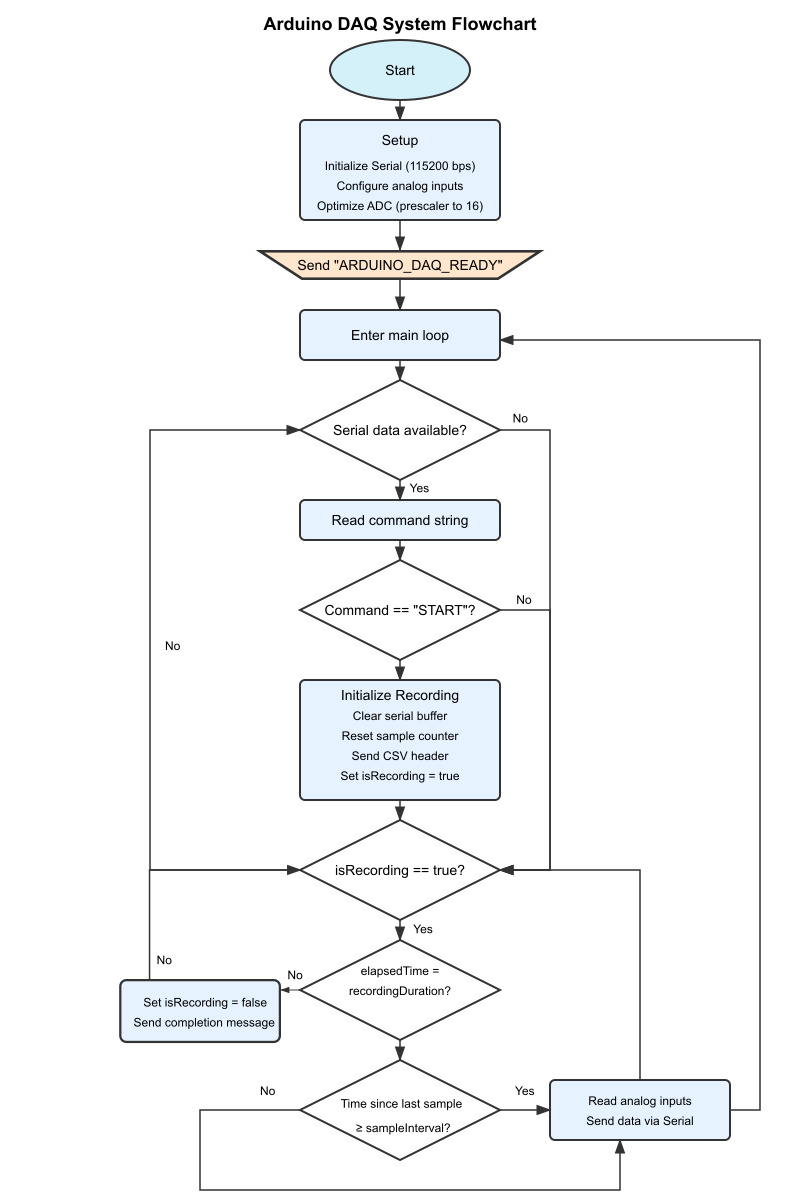
\includegraphics[width=0.95\textwidth]{chapters/methodology/ArduinoDAQ/flowchart_Arduino_code.png}
    \caption{Flowchart Arduino DAQ C++ program}
    \label{fig:arduinoPseudoCodeFlowchart}
\end{figure}

% FSM Arduino LOOP
\begin{figure}[htbp] %h-ere t-op b-ottom p-page (separate) -good to allow all htbp to give the compiler more options
  \centering
  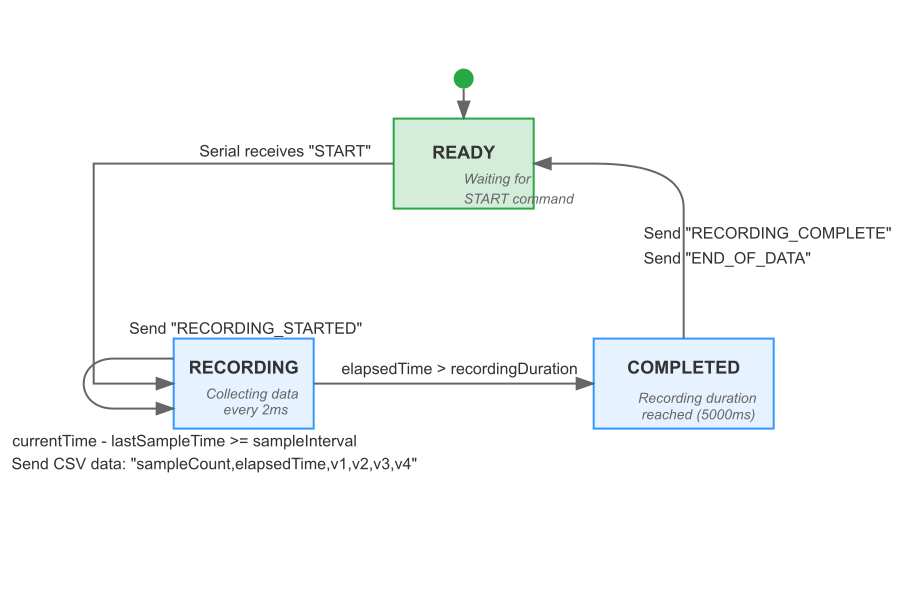
\includegraphics[width=0.95\textwidth]{chapters/methodology/ArduinoDAQ/arduino_loop_FSM.png}
  \caption{FSM Arduino C++ LOOP}
  \label{fig:arduinoFSM}
\end{figure}

%%% Arduino CPP pseudocode
\begin{lstlisting}[style=cstyle, caption=Arduino DAQ PseudoCode, label=lst:arduinoPseudoCode]
  recordingDuration = 5000 // for how long to record in milliseconds
  
  minSampleInterval = 2    // control how fast to sample to avoid
                           // relying on Arduino performance
  // Initialize serial communication
  // Initialize analog inputs
  // Setup ADC

  // Inform PC listening on Serial Connection: Arduino is ready to record
  Serial.print("Arduino_DAQ_Ready")
  // enter the loop 
  void loop(){
    //listen for command from PC script:
      String command = Serial.read()
    //set system state
    if (command == "START"){
      // Send header of csv
      Serial.println("Sample,Time(ms),A0(V),A1(V),A2(V),A3(V)")
      // keep track of system state
      state = recording
      // keep time
      startTime = currentTime()
      // send confirmation
      Serial.println("recording in progress")
      }
    // check if recording
    if (state == recording){
      // check if within recording period
      currentTime = currentTime()
      elapsedTime = currentTime - startTime
      if(currentTime <= recordingDuration){
        // Also check not recording too fast  
        if(currentTime - lastSampleTime >= minSampleInterval){
          sampleCount++;
          // Start each row with sample count and time of sample
          String currentCSVrow = String(sampleCount) , string(elapsedTime)
          // Multiplex through all analog inputs 
          for (int = 0;i<4;i++){
            //read raw values
            rawValue = analogRead(analogInputs[i]);
            // compute real value
            voltage = rawValue * 5/1023
            // add value to current row to send
            currentCSVrow += String(voltage)
            }
          // Send completed row to PC
          Serial.println(currentCSVrow)
          }
        }
      }
  // end recording
  else{
    state = notRecording
    // tell PC recording finished
    Serial.println("Recording_finished")
    }
}
\end{lstlisting}

\paragraph{Sampling Rate Details}
Several factors restrict the sampling rate:

\subparagraph{Sample Interval Setting}
The most direct limitation is the \texttt{sampleInterval} constant set to 2ms in the code. It was meant to avoid having random sampling rates based on the number of computations required. This means samples are taken no more frequently than every 2 milliseconds (500 Hz theoretical maximum) of all four channels. The "jump" to sample the next channel is not limited in the code, but it will take 13 clock cycles, (ie. around 13µs at 1MHz ADC clock) to switch to the next channel.

\subparagraph{ADC Prescaler Configuration}
The ADC prescaler is set to 16 (from the default of 128) with this line:
\begin{verbatim}
ADCSRA = (ADCSRA & 0xF8) | 0x04;
\end{verbatim}
This increases the ADC clock to 16MHz/16 = 1MHz. With each conversion taking 13 ADC clock cycles, the theoretical maximum sampling rate is about 76.9kHz for a single channel.


\subparagraph{Serial Transmission Overhead}
Each sample requires formatting and sending data over serial:
\begin{verbatim}
String dataString = String(sampleCount) + "," + String(elapsedTime);
// ... format and add voltage values ...
Serial.println(dataString);
\end{verbatim}
This string creation and serial transmission takes some time to process as mentioned earlier.

\subparagraph{Serial Baud Rate}
The code uses 115200 bps, which limits how quickly data can be transmitted. Each sample in this format might be around 30-40 bytes, which means \texttildelow 3000-3800 samples/second theoretical maximum throughput.

\subparagraph{String Operations}
The use of the Arduino \texttt{String} class is memory-intensive and can cause fragmentation over time, potentially causing the slowdowns noticed during testing with larger timeframes (and longer strings).

%
%   Python Script section
%
\subsubsection{Python Script}
\label{subsub:DAQpython}
The digitized signal must be interpreted and saved on the PC. This is done via a python script which listens to the Serial port from the arduino. The signal then also required cleaning from RF interference discovered during testing. In Figure~\ref{fig:pythonFlowchart} a flowchart is produced showing the way the script works: after initial setup that sets up the Serial Communication, the script waits for a "DAQ\_READY" signal from the Arduino. Once this is received, a csv file is created and the script sends a "START" signal which the Arduino interprets and starts sampling and sending the data. The script receives each line and saves it in the new CSV, and continues to record data until the Arduino sends a "RECORDING\_COMPLETE" signal - which will happen when the recordingDuration is reached. At this point the python script  performs the following post-processing steps:

\paragraph{The filter\_and\_save\_data()} function' purpose is mainly to correctly interpret the CSV. It takes a csv with the raw voltage values, saves them into a Pandas DataFrame for easier manipulation and sends each channel to the apply\_lowpass\_filter() function which will be described below. filter\_and\_save\_data() pseudocode is produced in Listing \ref{lst:pythonFilterAndSave}.

% Flowchart of Python Script
\begin{figure}[ptb] 
  \centering
  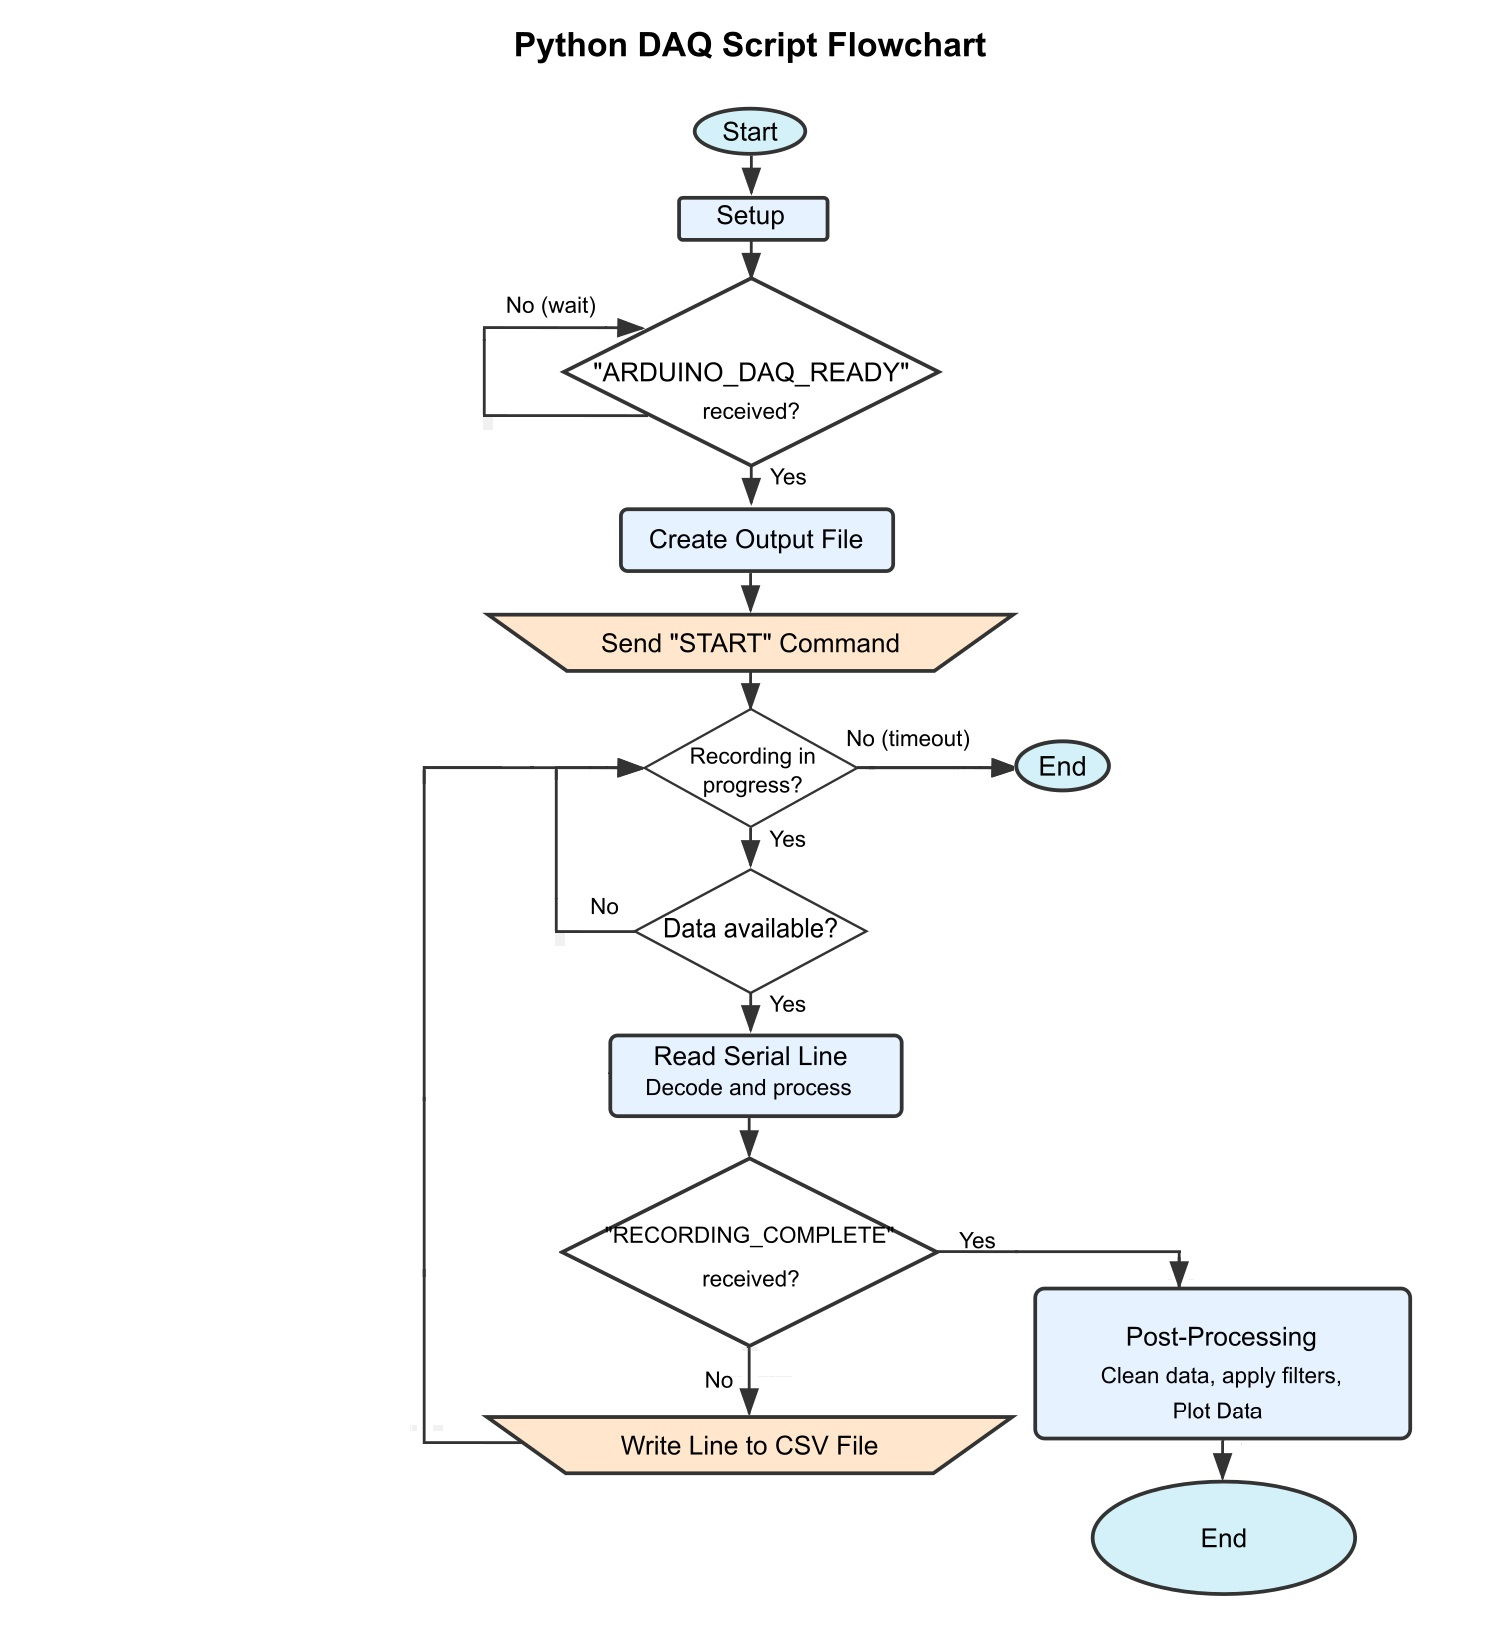
\includegraphics[width=0.95\textwidth]{chapters/methodology/ArduinoDAQ/python_serial_receive.jpg}
  \caption{Python Script Flowchart}
  \label{fig:pythonFlowchart}
\end{figure}

%%% Python Filter and save data pseudocode
\begin{lstlisting}[style=cstyle, caption=Python filter\_and\_save\_data() PseudoCode, label=lst:pythonFilterAndSave]
  FUNCTION filter_and_save_data(filename)
  // Load data from CSV file into a table structure
  data_table = READ_CSV(filename)
  
  // Streamline the data by converting text to numbers
  FOR EACH column IN data_table
      CONVERT column values to numeric type
      IF conversion fails for any value
          REPLACE with NaN (Not a Number)
  END FOR
  
  // Remove any rows containing NaN values
  REMOVE all rows with NaN values from data_table
  
  // Calculate sampling frequency
  time_differences = CALCULATE differences between consecutive time values
  typical_time_difference = FIND median of time_differences
  sampling_frequency = 1000.0 / typical_time_difference  // Convert ms to Hz
  
  // Process each data channel
  channel_list = ["A0(V)", "A1(V)", "A2(V)", "A3(V)"]
  
  FOR EACH channel_name IN channel_list
      IF channel_name EXISTS in data_table
          filtered_values = APPLY_LOWPASS_FILTER(original_values, sampling_frequency)
          ADD new column named channel_name + "_filtered" with filtered_values
      END IF
  END FOR
  
  // Save results to new file
  new_filename = REMOVE_EXTENSION(filename) + "_filtered.csv"
  WRITE data_table TO new_filename
  
  RETURN new_filename
END FUNCTION
\end{lstlisting}

\paragraph{The apply\_lowpass\_filter()} function was created and integrated into the script once it was observed that the RED testbench used was introducing noise as seen in Figure \ref{fig:sigNoise}. The benefit of using an already built testbench that could place the light at exact positions repeatedly, meant it would make sense to accept the noise and just filter the data, as the signal of interest was very low frequency while the noise was around 170kHz. The filter could be relatively simple, due to the large frequency difference between noise and signal. A 4th order Butterworth IIR filter was deemed acceptable and a low cut-off frequency of 1Hz or 2Hz was used for the static readings. This was found to be acceptable for the test involving light location at a frequency of 0.2Hz the transition of the light from one position to another was still visibly sharp. The post-processing is not the only reason light transition would not appear instantaneous on the Voltage graph, another reason is the amplification circuit which has a 1Hz cut-off frequency via the feedback capacitor on the secondary-amplification OpAmp circuit. \label{LowPassFilter}
The pseudocode of the function that creates the low-pass digital filter and filters the data is reproduced in Listing \ref{lst:pythonLowPassFilter}. The butter() function from the library signal is used, from the scipy package~\cite{RefWorks:butter} which is a free and open source library offered to the scientific community. Before feeding the cut-off frequency to the filter, it is normalized to the Nyquist rate, which means it is between 0 (DC) and 1 (Nyquist frequency), and therefore the filter can be applied no matter the sampling rate. As Schafer and Oppenheim explain in "Discrete-Time Signal Processing" Third Edition:
"The frequency scaling or normalization in the transformation from $ X_s(j\Omega) \text{ to } X(e^{j\omega})$ is directly a result of the time normalization in the transformation from $x_s(t) \text{ to } x[n]$"~\cite[p.171]{RefWorks:oppenheim2013discrete-time}.
When creating a digital filter, this normalization becomes crucial because in the continuous-time domain, frequencies are measured in Herz and in the discrete-time domain, frequencies become relative to the sampling rate.
The relationship between these two frequency domains is given by $\omega = \Omega T$, where:

\begin{itemize}
    \item $\omega$ is the normalized digital frequency (radians/sample)
    \item $\Omega$ is the analog frequency (radians/second)
    \item $T$ is the sampling period (seconds)
\end{itemize}

%%%%%%%%%%%%%%
However, when implementing IIR filters like the Butterworth filter used for our purpose, the bilinear transformation is employed to convert from the continuous-time domain to the discrete-time domain. This transformation introduces frequency warping, where the relationship between the analog and digital frequencies becomes:

$$\omega = 2 \arctan(\Omega T_d/2)$$

where $T_d$ is the sampling period. This non-linear relationship compresses the infinite analog frequency range $(-\infty, \infty)$ into the finite digital frequency range $(-\pi, \pi)$. The warping effect is more pronounced at higher frequencies, meaning that in our case it would not be noticeable \cite[p.529-530]{RefWorks:oppenheim2013discrete-time}.

A critical property of the bilinear transformation is stability preservation. In the analog domain, a stable system has all poles in the left half of the s-plane reproduced in Figure \ref{fig:unitCircle}. The bilinear transformation maps the entire left half of the s-plane to the interior of the unit circle in the z-plane. This ensures that the 4-pole Butterworth filter, which is stable in the continuous-time domain, remains stable when converted to its discrete-time equivalent. 
%%%%%%%%%%%%%%%%%
% unit circle
\begin{figure}[htbp] 
  \centering
  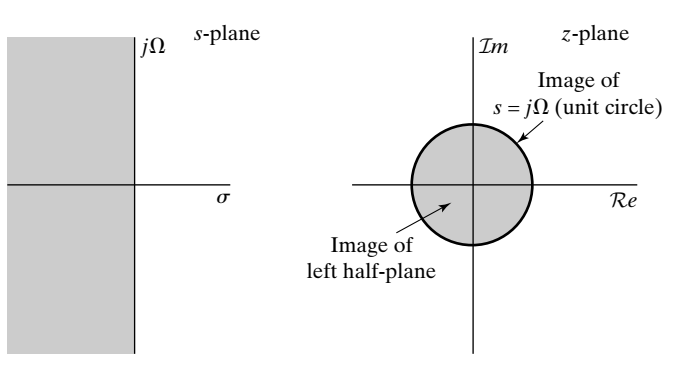
\includegraphics[width=0.7\textwidth]{chapters/methodology/ArduinoDAQ/oppenheimMappingCircle.png}
  \caption{Mapping of the s-plane onto the z -plane using \\ the bilinear transformation~\cite[p.130]{RefWorks:oppenheim2013discrete-time}}
  \label{fig:unitCircle}
\end{figure}

The filter Frequency Response was reproduced in Figure~\ref{fig:filterResponse} using the scipy.signal\-.freqz() method. The actual implementation uses filtfilt() which applies the filter twice, effectively doubling the filter order~\cite{RefWorks:2025filtfilt}. This affects the transition steepness and phase response. The Discrete-Time Transfer Function is reproduced in Equation \ref{DTFT-TF}.
% Filter Response equation
\begin{equation} \label{DTFT-TF}
  \begin{split}
    H(e^{j\omega}) = \frac{b[0] + b[1]e^{-j\omega} + b[2]e^{-j2\omega} + b[3]e^{-j3\omega} + b[4]e^{-j4\omega}}{a[0] + a[1]e^{-j\omega} + a[2]e^{-j2\omega} + a[3]e^{-j3\omega} + a[4]e^{-j4\omega}}
  \end{split}
\end{equation}
\addequation{Frequency Response of 4th-order Butterworth low-pass filter with 2.0 Hz cutoff}


%% APPLY_LOW_PASS_FILTER ()  PseudoCODE
\begin{lstlisting}[style=cstyle, caption=Python apply\_lowpass\_filter() PseudoCode, label=lst:pythonLowPassFilter]
  from scipy import signal
  FUNCTION apply_lowpass_filter(data, sampling_rate)
    // set hardcoded filter values
     cutoff_freq = 2;
     filter_order = 4;
    // calculate Nyquist Frequency and Normalized cut_off
    nyquist = 0.5 * sampling_rate;
    norm_cutoff = cutoff_freq / nyquist;
    // generate numerator b and denominator a polynomials 
    b, a = signal.butter(filter_order, norm_cutoff, filterType = LOW);
    // filter the data
    filtered_data = filter(b,a,data);

    return filtered_data;

\end{lstlisting}

% Filter Response (applied once)
\begin{figure}[htbp] 
  \centering
  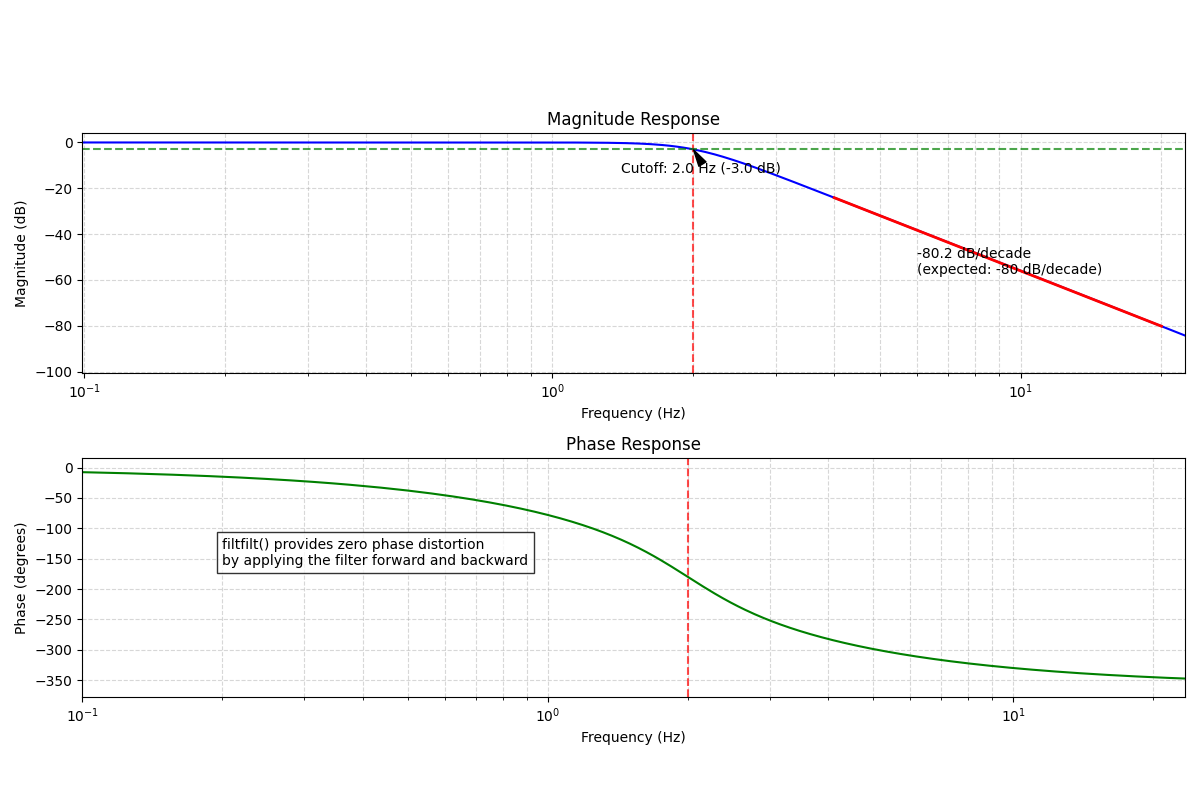
\includegraphics[width=1\textwidth]{chapters/methodology/ArduinoDAQ/filter_response.png}
  \caption{Frequency Response of 4-pole Butterworth Low-Pass Filter (Cutoff: 2.0 Hz, Order: 4, Fs: 500 Hz)}
  \label{fig:filterResponse}
\end{figure}

\subsection{Testing Strategy}
The testing was done incrementally with each new version of the program, many tests were carried out as the development was dependent on both C++ code on the Arduino and the Python script on the PC to somewhat work together. At first the C++ program was tested by listening to the output in the Serial Monitor of the Arduino IDE and sending commands the same way. Debug Serial.println() lines were used to ensure the loop on the Arduino was in the correct state. Once the C++ program seemed to somewhat work as intended, the Python script was implemented to send / receive. 

\subsection{Evaluation of design}
The design was tested iteratively while making changes to the code with a signal generator at first to simulate a stead known input signal and compare readings on the Arduino IDE Serial Monitor. Once the Python script was fully working, tests were performed again for the python script's ability to read the values sent correctly. An issue was identified where sometimes the Arduino would send the column headers not at the beginning of the CSV and these lines had to be cleaned manually. This could be due to Serial buffer issues but was not investigated. Later an attempt was made to perform the cleaning programmatically by creating a function in the script to do so.

